\documentclass[12pt,compress]{beamer}
\usepackage{amsmath}
\usepackage{url}
\usepackage{ucs}
\usepackage[utf8x]{inputenc}
\usepackage[ngerman]{babel}
\usepackage{ulem}  % sout
\usepackage{multicol}
\usepackage{comment}

% Manual syntax highlighting
\newcommand{\synfunc}   [1]{\color{blue!50!black}#1\color{black}}
\newcommand{\synstr}    [1]{\color{red!50!black}#1\color{black}}
\newcommand{\synvar}    [1]{\color{purple!50!black}#1\color{black}}
\newcommand{\synclass}  [1]{\color{green!50!black}#1\color{black}}
\newcommand{\syncomment}[1]{\color{blue!20!black}#1\color{black}}
\newcommand{\syncool}   [1]{\color{beamer@blendedblue}#1\color{black}}
\newcommand{\synoder}      {\ \ \color{black}$\vee$\ \ }
\newcommand{\hr}        {\rule[4pt]{\textwidth}{0.1pt}\\}
\newcommand{\hicolor}   [1]{\color[rgb]{0.6,0.2,0.8}#1\color{black}}
\newcommand{\synhilight}[1]{\hicolor{\textbf{#1}}}

\newcommand{\doofcomment}{\ \ \syncomment{\# :-(}}
\newcommand{\gutcomment} {\ \ \syncomment{\# :)}}

\title{Steganographie}
\author{Ingo~Blechschmidt, \\ Michael~Hartmann} %~\texttt{<iblech@web.de>},\\\hbox{Michael~Hartmann~\texttt{<michael.hartmann@as-netz.de>}}}
\institute{Linux User Group Augsburg e.\,V.}
\date{4. Oktober 2006}

\usetheme{Warsaw}  %Warsaw, Berkeley?
\usecolortheme{seahorse}
\usefonttheme{serif}
\useinnertheme{rectangles}
\usepackage{bookman}
\setbeamercovered{transparent}

\begin{document}

\frame{\titlepage}

\frame[t]{
  \frametitle{Inhalt}
  \tableofcontents
}

\section{Grundlagen}

\subsection[Def.]{Definition der Steganographie}

\frame[t]{
  \frametitle{Was ist Steganographie?}

  \begin{block}{Definition}
    Steganographie ist die Wissenschaft der verborgenen Übermittlung von Informationen.
  \end{block}

  \vfill

  Einsatzgebiete:
  \begin{itemize}
    \item{Sprache}
    \item{Digitale Medien}
    \item{Sport}
    \item{Kopierschutz}
  \end{itemize}
}

\subsection[Beispiele]{Beispiele für Steganographie}
\frame[t]{
  \frametitle{Beispiele für Steganographie}
  
  \begin{itemize}
    \item{Handzeichen beim Volleyball und Fußball}
    \item{Einsagen bei Ausfragen}
    \item{Versteckte Daten in Bildern, Audio- und Videodateien}
    \item{Umgehen von Servereinschränkungen (versteckte MP3 in Bildern)}
    \item{Passiver Kopierschutz $\rightarrow$ Wasserzeichen}
    \item{Verfassen von Briefen mit "`Geheimtinte"'}
  \end{itemize}
}

\subsection[Geschichte]{Historische Anwendungen der Steganographie}
\frame[t]{
  \frametitle{Historische Anwendungen}

  \begin{itemize}
    \item{Demeratus' Warnung an Sparta vor Angriff der Xerer}
    \item{Tätowierung von kahlrasierten Köpfen}
    \item{microdots: winzige Punkte, denen man keine Beachtung schenkt (1941 in Deutschland erfunden)}
    \item{Verbot von Postsendungen mit u.a. Schachaufgaben, Kreuzworträtseln, Zeitungsausschnitten, Strickmuster in den USA und England während des Zweiten Weltkriegs}

  \end{itemize}

  \vfill\hfill
  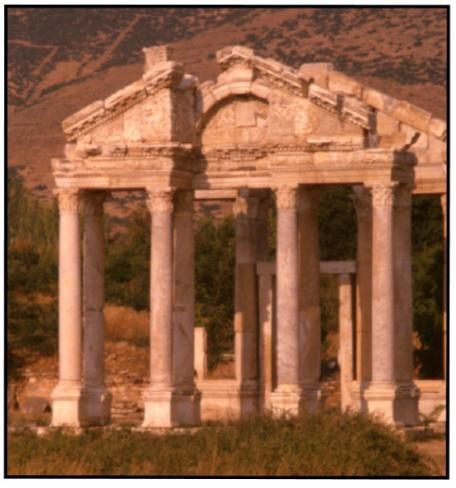
\includegraphics[scale=0.22]{images/tempel.jpg}
}

\subsection[Abgrenzung]{Abgrenzung zur Verschlüsselung}
\frame[t]{
  \frametitle{Abgrenzung zur Verschlüsselung}

  \begin{itemize}
    \item{Erregung von Verdacht durch verschlüsselte Nachrichten}
    \item{Verheimlichung von Informationsübermittlung durch Steganographie}
    \item{Steganographie kaum erkennbar}
    \item{Einfache bis sehr komplexe\\steganographische Algorithmen}
  \end{itemize}

  \vfill\hfill
  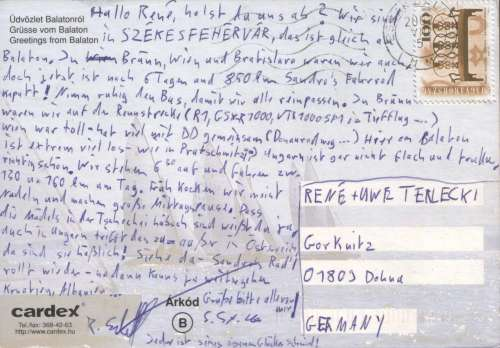
\includegraphics[scale=0.3]{images/postkarte.jpg}
}

\subsection[Mathematik]{Mathematischer Hintergrund}
\frame[t]{
  \frametitle{Mathematischer Hintergrund}

  \begin{block}{Informationsgehalt eines Zeichens}
    \[
      I(x) := -\log_2 P(x); \qquad [1 \,\mathrm{bit}]
    \]
  \end{block}
  
  \begin{block}{Entropie: Zu erwartender Informationsgehalt}
    \[
      E(I) := \sum\limits_{x \in \Sigma} P(x) \cdot I(x);
    \]
  \end{block}

  \vspace*{-1em}
  \begin{tabbing}
    asdfff \= \kill
    $x$:      \> ein bestimmtes Zeichen \\
    $\Sigma$: \> Menge aller vorkommenden \\ \> Zeichen \\
    $P(x)$:   \> Wahrscheinlichkeit \\ \> des Auftretens von $x$ \\
  \end{tabbing}

  \vspace*{-9em}\hfill 
  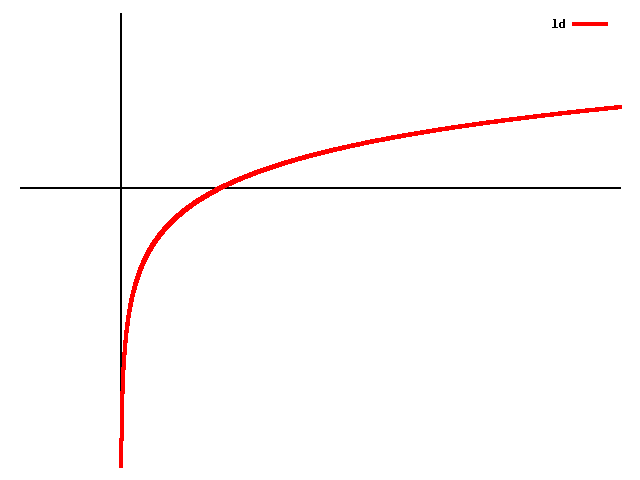
\includegraphics[scale=0.15]{images/log.png}
}

\frame[t]{
  \frametitle{Beispiel}

  \begin{block}{Definitionen}
    \[
      \renewcommand{\arraystretch}{1.2}
      \begin{array}{rcl}
        I(x) &:=& -\log_2 P(x); \\
        E(I) &:=& \sum\limits_{x \in \Sigma} P(x) \cdot I(x);
      \end{array}
    \]
  \end{block}
  
  \[ 
    \begin{array}{rcl}
      M      &=& \left(a,l,l,e,s\right); \\
      \Sigma &=& \left\{a,e,l,s\right\};
    \end{array}
  \]
  
  \[
    \renewcommand{\arraystretch}{1.2}
    \begin{array}{rcl}
      I(a) = I(e) = I(s) &=& -\log_2 \frac{1}{5} \approx 2{,}32 \,\mathrm{bit}; \\
      I(l) &=& -\log_2 \frac{2}{5} \approx 1{,}32 \,\mathrm{bit};
    \end{array}
  \]

  \[
    E(I) \approx 3 \cdot \frac{1}{5} \cdot 2{,}32 \,\mathrm{bit} + \frac{1}{5} \cdot 1{,}32 \,\mathrm{bit} \approx 1{,}67 \,\mathrm{bit};
  \]
}

\frame[t]{
  \frametitle{Eigenschaften der Entropie}

  \begin{itemize}
    \item Je seltener ein Zeichen, desto höherer Informationsgehalt
    \item Spezialfall bei gleicher Häufigkeit aller Zeichen: \\
          $P(x_1) = P(x_2) = \cdots = P(x_n) =: p$ \\
          $I(x_1) = I(x_2) = \cdots = I(x_n) = -\log_2 p =: i$ \\
          $E(I) = i$ \\\ \\

          Beispiel: \\
          $M = (1,2,3,4,1,2,3,4,1,2,3,4);$ \\
          $p = \frac{1}{4};$ \\
          $E(I) = i = -\log_2 \frac{1}{4} = 2 \,\mathrm{bit};$

    \item Maximale Entropie bei $\Sigma = \left\{ 0, 1 \right\}^8$: \\
          $E(I) = 8 \,\mathrm{bit};$
  \end{itemize}
}

\frame{
  \frametitle{Praktische Entropiebestimmung}
  \begin{center}\Huge \scalebox{2}{\textsl{Live-Demo}}\end{center}
}

\frame{
  \frametitle{Praktische Entropiebestimmung}

  \begin{center}
    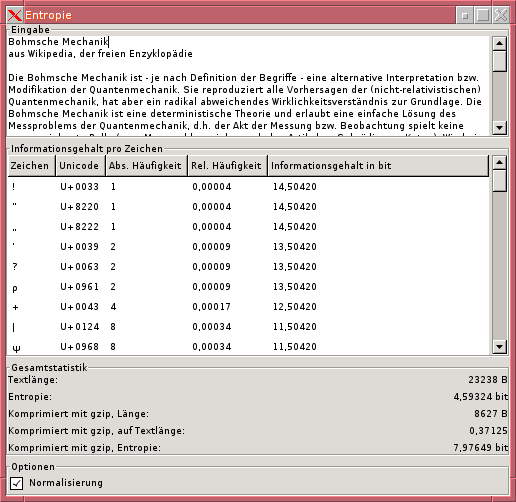
\includegraphics[scale=0.4]{images/entropy-pl.png} \\\ \\
    \footnotesize \texttt{entropy.pl} von \url{http://xrl.us/luga-entropy}
  \end{center}
}

\frame[t]{
  \frametitle{Praktische Entropiebestimmung}

  \begin{itemize}
    \item Beispielimplementierung \texttt{entropy.pl} zur Bestimmung von
          Informationsgehalt und Entropie
    \item Aufruf mit: \\
          \texttt{\$ perl entropy.pl} oder: \\
          \texttt{\$ perl entropy.pl corpus.txt} \\
    \item Benötigte nicht-Standard-Perl-Module: \\
          Compress::Zlib, Gtk2

    \item Installation über: \\
          \scriptsize
          \texttt{\# apt-get install libcompress-zlib-perl libgtk2-perl} oder: \\
          \texttt{\# perl -MCPAN -eshell \\
          > install Compress::Zlib \\
          > install Gtk2}
  \end{itemize}
}

\section[Anwendungen]{Anwendungen}

\subsection{Verzeichnisse}
\frame[t]{
  \frametitle{Verzeichnisse als Trägermedium}

  \scriptsize
  \texttt{%
    \$ ls -l\\
    -rw-rw-rw- 1 user group 3237\textbf<2>{2} 01-Mathematik.txt\\
    -rw-rw-rw- 1 user group 6381\textbf<2>{4} 02-Physik.txt\\
    -rw-rw-rw- 1 user group \ 483\textbf<2>{1} 03-Chemie.txt\\
    -rw-rw-rw- 1 user group \ 112\textbf<2>{9} 04-Biologie.txt\\
    -rw-rw-rw- 1 user group 1003\textbf<2>{7} 05-Musik.txt\\
    -rw-rw-rw- 1 user group 5700\textbf<2>{1} 06-Kunst.txt\\
  }
}

\subsection{Text}
\frame[t]{
  \frametitle{Text als Trägermedium}

  \vspace*{3em}

  \scalebox{1.2}{
    \vbox{
      \begin{tiny}
	\texttt{%
	  \textbf<2>{L}inux ist ein freies und plattformübergreifendes Betriebssystem, das  \\
	  \textbf<2>{U}NIX ähnlich ist. Schon bald nach Beginn der Entwicklung liefen viele \\
	  \textbf<2>{G}NU-Tools, beispielsweise cat, echo, bash uvm. Nach kurzer Zeit wurde \\
	  \textbf<2>{a}uch ein Maskottchen für das noch junge System gefunden: ein Pinguin. \\
	}
      \end{tiny}
    }

  }
  
  \vfill
  \only<2>{
    \begin{itemize}
      \item{Relativ einfach zum Lesen und Erstellen}
      \item{Viele Algorithmen denkbar}
      \item{Kaum nachvollziehbar}
    \end{itemize}
  }
}

\subsection{Bilder}
\frame[t]{
  \frametitle{Bilder als Trägermedium}

  \begin{itemize}
    \item{Verbergen von Daten durch Veränderung von Farben oder Verzerrung}
    \item{%
      Farbänderung: \\
      Nutzung der Least Significant Bits (LSB) als Träger
      $\rightarrow$ minimale (kaum wahrnehmbare) Veränderung des Bildes \\
      \ \\
      $10001010_2$ ($= 1\cdot 2^7 + 1\cdot 2^3 + 1\cdot2^1 = 138$) → \\
      $10001011_2$ ($= 1\cdot 2^7 + 1\cdot 2^3 + 1\cdot2^1 + 1\cdot2^0 = 139$)
    }

    \item{Veränderung der LSB prinzipiell auch bei Audiodateien möglich}
    \item{Verzerren: \\ Geringfügige, systematische Verzerrung abhängig von den zu versteckenden Daten}
  \end{itemize}
}

\frame[t]{
  \frametitle{stega.pl -- Funktionsweise}

  \begin{itemize}
    \item{Beispielimplementierung stega.pl von \url{http://xrl.us/lugastega}}
    \item{Einbettungsalgorithmus: \\
          Veränderung der drei LSB der Rot-, Grün- und Blaufarbwerte jedes Pixels
          (von links nach rechts und oben nach unten)
         }
    \item{Extraktionsalgorithmus: \\
          Auslesen der drei LSB des Rot-, Grün- und Blaufarbwerte jedes Pixels
          (von links nach rechts und oben nach unten)
         }
    \item{Kapazität:
          \[ \frac{\text{Höhe} \cdot \text{Breite} \cdot 3 \,\mathrm{bit}}{8
          \,\frac{\mathrm{bit}}{\mathrm{B}}} \] \\
          \footnotesize
          (Höhe, Breite in Pixeln; z.B.: 50x50px: 0,9 KiB)
         }
  \end{itemize}
}

\frame[t]{
  \frametitle{stega.pl -- Nutzung}

  \begin{itemize}
    \item{Daten in Bild verstecken: \\
          \footnotesize
          \texttt{%
            \$ ./stega.pl \textbackslash\\
            \ \ \ \ --mode=embed \textbackslash\\
            \ \ \ \ --input=originalbild.png \textbackslash\\
            \ \ \ \ --output=verändertes-bild.png
          }
         }
    \item{Daten aus Bild extrahieren: \\
          \footnotesize
          \texttt{%
            \$ ./stega.pl \textbackslash\\
            \ \ \ \ --mode=extract \textbackslash\\
            \ \ \ \ --input=verändertes-bild.png
          }
         }
  \end{itemize}
}

\frame{\begin{center}%
  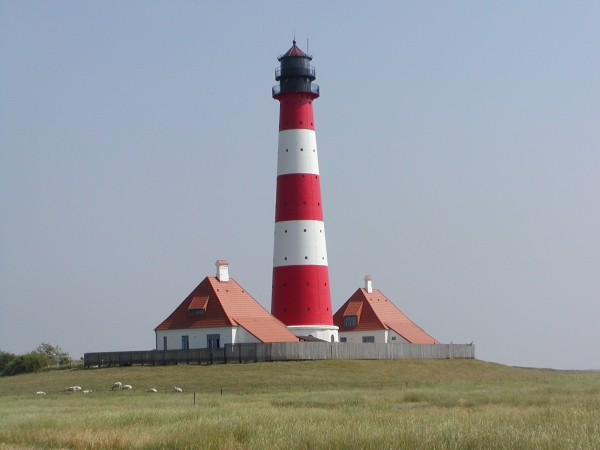
\includegraphics[scale=0.4]{images/leuchtturm-vorher.png} \\\ \\%
  \footnotesize unverändertes Bild \textcolor{white}{g}%
\end{center}}
\frame{\begin{center}%
  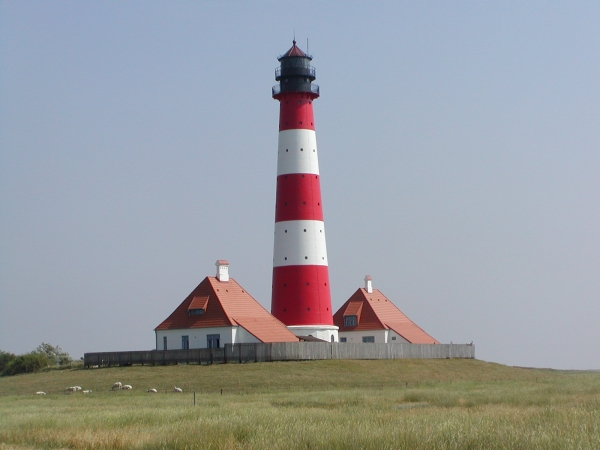
\includegraphics[scale=0.4]{images/leuchtturm-nachher.png} \\\ \\%
  \footnotesize steganographisch verändertes Bild%
\end{center}}

\frame{\begin{center}
  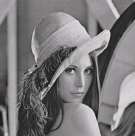
\includegraphics{images/lena-vorher.png} \\\ \\
  \footnotesize Lena, Original
\end{center}}
\frame{\begin{center}
  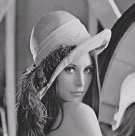
\includegraphics{images/lena-nachher.png} \\\ \\
  \footnotesize Lena, steganographisch verändert
\end{center}}

\frame{\begin{center}
  
\includegraphics{images/raster-vorher.png} \\\ \\
  \footnotesize Raster, Original
\end{center}}
\frame{\begin{center}
  
\includegraphics{images/raster-nachher.png} \\\ \\
  \footnotesize Raster, steganographisch verändert
\end{center}}

\frame[t]{
  \frametitle{Beispielimplementierung}

  \begin{itemize}
    \item steghide von Stefan Hetzl (\url{http://steghide.sourceforget.net/})
    \item Einbettung in Bilder (JPEG und BMP) und Audiodateien (WAV, AU)
  \end{itemize}

  \scriptsize
  \begin{enumerate}
    \item{\texttt{steghide embed -cf \ \ träger.jpeg -ef geheim.txt}}
    \item{\texttt{steghide extract -sf träger.jpeg}}
  \end{enumerate}
}

\subsection[TTL]{Variation des TTL-Wertes}
\frame[t]{
  \frametitle{Variation des TTL-Wertes von IP Paketen}

  \begin{itemize}
    \item{Time-to-Live: Zahl im Header von IP Paketen, die nach jedem passierten Rechner dekrementiert wird}
    \item{Verhindern von "`Endlosrouting"' durch TTL (A schickt Paket an B, B zurück zu A)}
    \item{Übermittlung von Daten durch unterschiedliche TTL-Werte in IP Paketen}
  \end{itemize}

  \vfill\hfill
  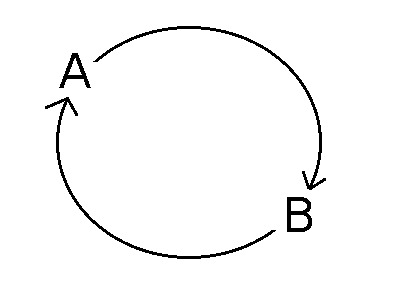
\includegraphics[scale=0.2]{images/ab.png}
}

\frame[t]{
  \frametitle{Beispiel: Variation des TTL-Wertes}

  Variation des TTL-Wertes nach einem (hier sehr einfachen) Algorithmus: \\

  \begin{itemize}
    \item{Zuordnung: \\ TTL des empfangenen Pakets $\rightarrow$ Buchstabe im Alphabet \\
          1 $\mapsto$ a,\\
          2 $\mapsto$ b,\\
          \ldots}
    \item{Beispiel-Route: Sender $\rightarrow$ Router $\rightarrow$ Empfänger:\\
      \begin{enumerate}
        \item{Sender schickt Paket mit TTL 13}
        \item{Router dekrementiert TTL auf 12}
        \item{Empfänger empfängt Paket mit TTL 12}
        \item{Interpretiert Paket als "`L"'}
      \end{enumerate}}
  \end{itemize}
}

\frame[t]{
  \frametitle{Beispiel: Variation des TTL-Wertes}

  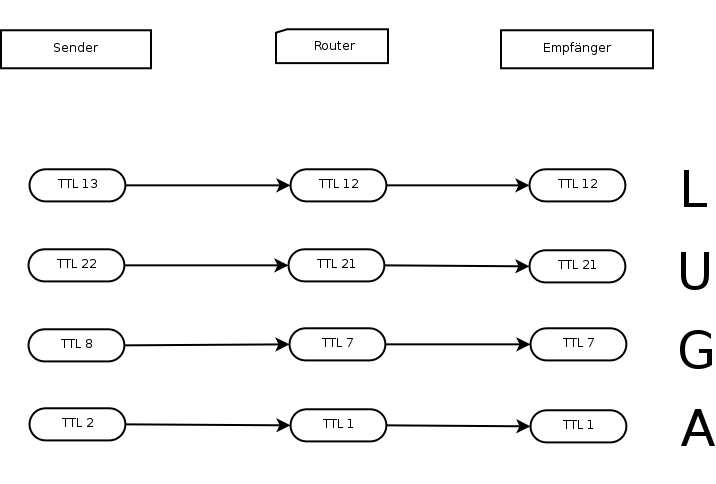
\includegraphics[scale=0.29]{images/ttl.png}
}
\subsection[DNS]{Domain Name Service (DNS)}
\frame[t]{
  \frametitle{Domain Name Service (DNS)}

  \hbox{\footnotesize$
    \left.
      \begin{array}{l}
        \text{1. Nicht-rekursiver} \\
        \text{2. Rekursiver} \\
        \text{3. Nicht-rekursiver}
      \end{array}
    \right\}
    \begin{array}{l}
      \text{Lookup auf nicht} \\
      \text{existente Domain}
    \end{array}
    \rightarrow
    \left\{
      \begin{array}{@{}ll}
        \text{NOERROR}  & := \texttt{0} \\
        \text{NXDOMAIN} & := \texttt{1} \\
        \text{NXDOMAIN} & := \texttt{1}
      \end{array}
    \right.
  $}

  \vfill
  \begin{itemize}
    \item Setzen eines Bits: \\
          \texttt{\$ \textbf{dig @ns bit-addr +recursive}} \\
    \item Abfragen eines Bits: \\
          \texttt{\$ \textbf{dig @ns bit-addr +norecursive}} →
          \begin{tabbing}
            NXDOMAIN? \= \kill
            NOERROR?  \> → \texttt{0} \\
            NXDOMAIN? \> → \texttt{1}
          \end{tabbing}
    \item \ldots mit \texttt{bit-addr} beispielsweise
          \texttt{1234.pugs-rules.de} für das 1234. Bit
  \end{itemize}
}

\frame{
  \frametitle{Beispielimplementierung}
  \begin{center}\Huge \scalebox{2}{\textsl{Live-Demo}}\end{center}
}

\frame[t]{
  \frametitle{Beispielimplementierung}

  \begin{itemize}
    \item Beispielimplementierung dnsx von \url{http://xrl.us/lugadnsx}
    \item Benötigtes nicht-Standard-Perl-Modul: \\
          Net::DNS

    \item Installation über: \\
          \scriptsize
          \texttt{\# apt-get install libnet-dns-perl} oder: \\
          \texttt{\# perl -MCPAN -eshell \\
          > install Net::DNS}
  \end{itemize}
}

\frame[t]{
  \frametitle{Speichern im DNS}

  \texttt{%
    \$ ./dnsx \textbackslash\\
    \ \ \ \ --nameserver=\textsl{Nameserveradresse} \textbackslash\\
    \ \ \ \ --domain=\textsl{Unbenutzte Domain} \textbackslash\\
    \ \ \ \ --mode=store
  }

  (dnsx liest von der Standardeingabe.)
}

\frame[t]{
  \frametitle{Holen aus dem DNS}

  \texttt{%
    \$ ./dnsx \textbackslash\\
    \ \ \ \ --nameserver=\textsl{Nameserveradresse} \textbackslash\\
    \ \ \ \ --domain=\textsl{Unbenutzte Domain} \textbackslash\\
    \ \ \ \ --mode=receive \textbackslash\\
    \ \ \ \ --length=\textsl{Länge der Daten}
  }

  (dnsx schreibt auf die Standardeingabe.)
}

\frame[t]{
  \frametitle{Anmerkungen zu dnsx}

  \begin{itemize}
    \item Wahl einer unbenutzten Domain als \texttt{--domain} zwingend
    \item Keine "`prinzipielle Korrektheit"' der Domain erforderlich; \\
          beispielsweise Möglichkeit von \texttt{--domain=weltklasse.9live}
    \item Unterdrücken der Debuggingmeldungen durch Umleitung der
          Standardfehlerausgabe
  \end{itemize}
}

\subsection[JitterBugs]{Tastaturverzögerung}
\frame[t]{
  \frametitle{Tastaturverzögerung mit JitterBugs}

  \begin{itemize}
    \item Verbergen von Information durch systematische Verzögerung von
          Tastenanschlägen durch ein externes Gerät zwischen Tastatur und
          Computer
    \item Mathematisches Prinzip:
          \begin{tabbing}
            $\Delta t$: \= \kill
            $\Delta t$: \> Zeitdauer zwischen zwei Anschlägen \\
            $T$:        \> Zeitfenster, bspw. $20 \,\mathrm{ms}$
          \end{tabbing}

          \ \\
          Übertragung von $0$? \\
          → Verzögerung so, dass $\Delta t$ durch $T$ teilbar

          \ \\
          Übertragung von $1$? \\
          → Verzögerung so, dass $\Delta t + \frac{T}{2}$ durch $T$ teilbar
  \end{itemize}
}

\frame[t]{
  \frametitle{Beispiel}

  \begin{itemize}
    \item Zeitdauer zwischen Anschlägen des Benutzers: \\
          $\begin{array}{cccc}
            42 \,\mathrm{ms}, &
            57 \,\mathrm{ms}, &
            19 \,\mathrm{ms}, &
            86 \,\mathrm{ms}
          \end{array}$
    \item Zeitfenster: $T = 20 \,\mathrm{ms}$
    \item Zu übertragende Information: $1011_2$
    \item Zeitdauer zwischen den Anschlägen nach künstlicher Verzögerung: \\
          $\begin{array}{cccc}
            \underbrace{60  \,\mathrm{ms}}_1, &
            \underbrace{70  \,\mathrm{ms}}_0, &
            \underbrace{20  \,\mathrm{ms}}_1, &
            \underbrace{100 \,\mathrm{ms}}_1
          \end{array}$
  \end{itemize}

  \vfill
  \begin{block}{Trotz verschiedenen Quellen von Rauschen\ldots}
    \ldots Detektierbarkeit solcher Verzögerungen übers Netzwerk! (!!)
  \end{block}
}

\frame{
  \begin{center}
    \Huge
    \scalebox{2}{\textsl{Live-Demo}}

    \vfill
    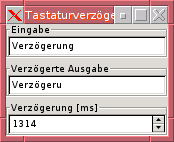
\includegraphics[scale=0.8]{images/keyboard-delay-pl.png}
  \end{center}
}

\frame{\begin{center}
  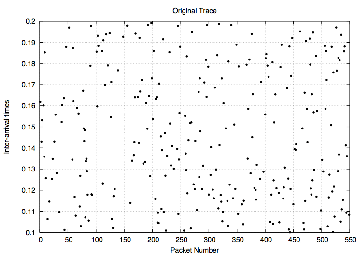
\includegraphics[scale=0.7]{images/jitterbugs-vorher.png} \\\ \\
  \footnotesize Ohne JitterBugs
\end{center}}
\frame{\begin{center}
  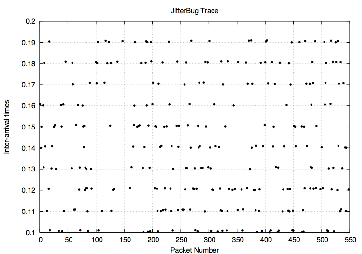
\includegraphics[scale=0.7]{images/jitterbugs-nachher.png} \\\ \\
  \footnotesize Mit JitterBugs
\end{center}}

\frame{\begin{center}\Huge \scalebox{2}{\textsl{Fragen?}}\end{center}}

\section{Quellen}
\subsection{Literatur}
\frame[t]{
  \frametitle{Literatur}

  \tiny
  \begin{itemize}
    \item{\url{http://arxiv.org/pdf/math.HO/0404335}}
    \item{\url{http://m19s28.vlinux.de/iblech/klasse11/Sonstiges/1337/LUGA/DNS.pdf.pdf}}
    \item{\url{https://db.usenix.org/events/sec06/tech/shah/shah_html/index.html}}
    \item{\url{http://www.expmath.org/expmath/volumes/11/11.3/Calude361_370.pdf}}
    \item{\url{http://www.petitcolas.net/fabien/publications/ieee99-infohiding.pdf}}
  \end{itemize}
}

\subsection{Bildquellen}
\frame[t]{
  \frametitle{Bildquellen}

  \tiny
  \begin{itemize}
    \item{\url{http://perl.plover.com/yak/presentation/samples/present.gif}}
    \item{\url{https://db.usenix.org/events/sec06/tech/shah/shah_html/index.html}}
    \item{\url{http://www.alte-geschichte.uni-hd.de/grafik/tempel1.jpg}}
    \item{\url{http://www.htwm.de/~sstiller/kroatien/Postkarte\%20Balaton\%202.jpg}}
    \item{\url{http://www.meganandjack.com/mt/archives/signals4.jpg}}
    \item{\url{http://www.petitcolas.net/fabien/publications/ieee99-infohiding.pdf}}
  \end{itemize}
}

\appendix
\frame{
  \begin{center}\Huge Bonus-Slides\end{center}
  \tableofcontents
  \vspace*{10em}
  \hfill\raisebox{0pt}[0pt][0pt]{\vspace*{10em}
\includegraphics[scale=0.20]{images/bonus.png}}
}

\section{Algorithmische Informationstheorie (AIT)}
\subsection{Algorithmische Information}
\frame[t]{
  \frametitle{Algorithmische Informationstheorie (AIT)}

  \begin{itemize}
    \item Problem am Entropiekonzept: \\
          Entropien von \\
          $00001111$ und \\
          $01101000$ gleich!
    \item Reihenfolge spielt beim Entropiekonzept keine Rolle!
    \item Lösung: Algorithmische Information -- \\
          Länge des kürzesten Programms einer bestimmten Programmiersprache,
          die die jeweilige Zeichenkette ausgibt

          \[
            H(x) := \operatorname{min} \left\{
              \left|p\right| \,|\,
              M(p) = x
            \right\}\!;
          \]

          $M(p)$: Ausgabe des Programms $m$
  \end{itemize}
}

\subsection{Vergleich zur Entropie}
\frame[t]{
  \frametitle{Vergleich zur Entropie}

  \begin{itemize}
    \item Beachtung der Reihenfolge durch die algorithmische Information
    \item Bessere Erfassung des anschaulichen \\ Konzepts \textsl{Ordnung}:
          \begin{tabbing}
            $00001111$: \= \kill
            $00001111$: \> 4 Nuller gefolgt von 4 Einsern \\
            $01101000$: \> Eine Null, zwei Einser, eine Null, \\\> eine Eins, drei Nuller
          \end{tabbing}
    \item Allerdings: Praktische Bestimmung von $H(x)$ mitunter schwierig, da
          Ausprobieren sehr vieler Programme notwendig
    \item \textsl{Weitreichende, hier nicht näher genannte Konsequenzen für die
          Mathematik!} \\
          \scriptsize
          Stichworte: G. Chaitin, CHAITINsche
          Kon\-stan\-te/Hal\-te\-wahr\-schein\-lich\-keit
          $\Omega$, \ldots
  \end{itemize}
}

\end{document}
